\documentclass[12pt]{article}
\setlength{\topmargin}{0cm}
\setlength{\headheight}{0cm}
\setlength{\headsep}{0cm}
\setlength{\topskip}{0cm}
\setlength{\oddsidemargin}{0cm}
\setlength{\evensidemargin}{0cm}
\setlength{\textheight}{8.5in}
\setlength{\textwidth}{6.5in}
\setlength{\footskip}{1.5cm}


\usepackage{epsfig}
%%%%%%%\usepackage{dcolumn}
\usepackage{graphics}
\usepackage{longtable}
\usepackage{subfigure}  % use for side-by-side figures
\usepackage{amssymb}
\usepackage{amsmath}
\usepackage{times}

% the following to make better pdf
% \usepackage{aaai}
\usepackage{times}

\begin{document}

\newcommand{\met}{\mbox{$\raisebox{.3ex}{$\not$}E_T$\hspace*{0.5ex}}} 
\newcommand{\mpt}{\mbox{$\raisebox{.3ex}{$\not$}p_T$\hspace*{0.5ex}}} 

\subsection{Suppressing QCD contributions to lepton + jets using $\alpha_T$}

Following the promising results of the $\alpha_{T}$ jet-balancing method previously described for the all-hadronic SUSY searches, it is a natural progression to look for extensions of this approach to the single-electron search, where a significant presence of QCD multi-jet backgrounds is expected.

The $\alpha_{T}$ variable is here defined as an N-object system where the set of objects is 1 electron and N-1 jets. This definition reproduces the kinematics of a di-jet system by contructing two pseudo-jets, which balance one another in $H_{T}$. The two pseudo-jets are formed from the combination of the N objects that minimizes the $\Delta H_{T} \equiv |H_{T,1} - H_{T,2}|$ of the pseudo-jets, and the resulting  $\alpha_{T}$ is
\begin{equation}
\alpha_{T} = \frac{1}{2} \frac{H_{T} - \Delta H_{T}}{M_{T}} =  \frac{1}{2} \frac{H_{T} - \Delta H_{T}}{\sqrt{H_{T}^{2}-MH_{T}^{2}}}.
\end{equation}

The basic selection for single electron events in the leptonic $\alpha_{T}$ approach has the follwoing requirements:
\begin{itemize}


\item Exactly one electron passing requirements as follows:
\begin{itemize}
\item $p_{T} >$ 20 GeV
\item $|\eta| <2.4$
\item Passes the Cut Based ID formed by simple, yet robust, variables (these are the $H/E$, the super-cluster (SC) - track matching variables $\Delta \phi$,$\Delta \eta$, and shower shape variable $\sigma_{i\eta i\eta}$, Tracker Isolation, ECAL Isolation and HCAL Isolation\footnote{The cut based ID selection cuts are chosen to correspond to an 80\% efficiency in the $W\rightarrow e\nu$ analysis.}). 
\end{itemize}
\item The event is vetoed if there are any muons passing the following requirements:
\begin{itemize}
\item $p_{T} >$ 15 GeV
\item $|\eta| <2.1$
\item Passes ID requirement: IsGlobalMuon
\end{itemize}
\item A jet is rejected if it is found close to a tight and isolated electron within $\Delta R$=0.5.
 The jet selection is as follows:
\begin{itemize}
\item $p_{T} >$ 20 GeV
\item $|\eta| <5$
\item EMF $<$0.9
\end{itemize}

\end{itemize}

The analysis uses data samples for the QCD multi-jet background processes produced with the full simulation production for Physics at 7TeV with CMS. The Monte Carlo datasets used are detailed in Table \ref{tab:datasets}. The available luminosity is shown, although the plots are normallised to 1pb$^{-1}$. We use the EMenriched and BCtoE samples which are designed to be enriched in electrons, in order to enhance statistics. In addition, as these samples only cover the region 20$<\hat{p_{T}}<$170 GeV/c, we include the inclusive QCD Jets sample for the region $\hat{p_{T}}>$170 GeV/c.

\begin{table}[h!]
\begin{center}
\begin{tabular}{|c|c|c|c|}
\hline
Data Set & N events & $\sigma$ (pb) & Equivalent luminosity (pb$^{-1}$)\\
\hline
QCD BCtoE [20$<\hat{p_{T}}<$30]& 432380  & 108330 & 3.99\\
QCD BCtoE [30$<\hat{p_{T}}<$80] & 840100 & 138762 & 6.05\\
QCD BCtoE [80$<\hat{p_{T}}<$170 & 682720 & 9422.4 &72.4\\
QCD EM Enriched [20$<\hat{p_{T}}<$30] & 6169999 & 1719150 & 3.59\\
QCD EM Enriched [30$<\hat{p_{T}}<$80] & 9054696 & 3498700 & 2.59\\
QCD EM Enriched [80$<\hat{p_{T}}<$170] & 2492814 & 134088 & 18.59\\
QCDJets $\hat{p_{T}}>$170 & 3132800 & 25470 & 122.99\\
\hline
\end{tabular}
\end{center}
\caption{\textit{The Monte Carlo datasets used to investigate the Delta ID Inversion method in QCD backgrounds. The available Lumniosity is shown, although plots produced are normalised to 1pb$^{-1}$ for the purpose of understanding near-reach of CMS.}}
\label{tab:datasets}
\end{table}

This section is dedicated to a first approach of commissioning the alphaT observable and study its behavior in pure fake electron events. It is therefore desirable to collect a suitable control sample which will be dominated by fake electrons and eliminate sources of prompt electron events (like W events).
One way to obtain such a sample is using the anti-selection method on electron ID variables which are less correlated with the missing transverse energy. In this section, we investigate the possibility of inverting the $\Delta \eta$(trk-SC) and $\Delta \phi$ (trk-SC) id cuts in the electron selection. The anti-selected events in this method are collected with electrons that pass all selection id criteria except the $\Delta \phi$ (trk-SC) and $\Delta \eta$(trk-SC) ones. 

In order to establish the anti-selection method above, we compare next the perfomance of the leptonic $\alpha_T$ as obtained from the control sample and the actual QCD events passing the electron criteria defined in the ``signal'' region. The cutflow for 1pb$^{-1}$ is shown detailing number of events at each step for QCD and W samples, for selected in Table Xa and for anti selected in TableXb. 



\begin{table}[h!]
\begin{center}
\begin{tabular}{|c|c|c|c|c|}
\hline
Cutflow & QCD EM enriched & QCD BC$\rightarrow e$ & QCDJets Pythia $\hat{p_{T}}$ &  W \\
\hline
All events & & & & \\
\hline
N($e^{-}$) $\geq$ 1 & & & &\\
\hline
N($jets$) $\geq$ 1 & & & &\\
\hline
HT > 100 GeV & & & &\\
\hline
HT > 180 GeV & & & &\\
\hline

\end{tabular}
\begin{tabular}{|c|c|c|c|}
\hline
Cutflow & QCD Total & W &\\
\hline
All events & & & \\
\hline
N($e^{-}$) $\geq$ 1 & & &\\
\hline
N($jets$) $\geq$ 1 & & &\\
\hline
\end{tabular}

\end{center}

\end{table}










As mentioned previously, SUSY events are expected to have high $H_{T}$. Therefore it is critical to understand the behaviour in leptonic $\alpha_T$ as a function of $H_{T}$. The plots in \ref{fig:AlphaTbyHT} show the normalised shape of distributions, both before an $H_{T}$ cut and the evolution with HT. The selected and anti-selected distributions agree very well.
\begin{figure}[h!]

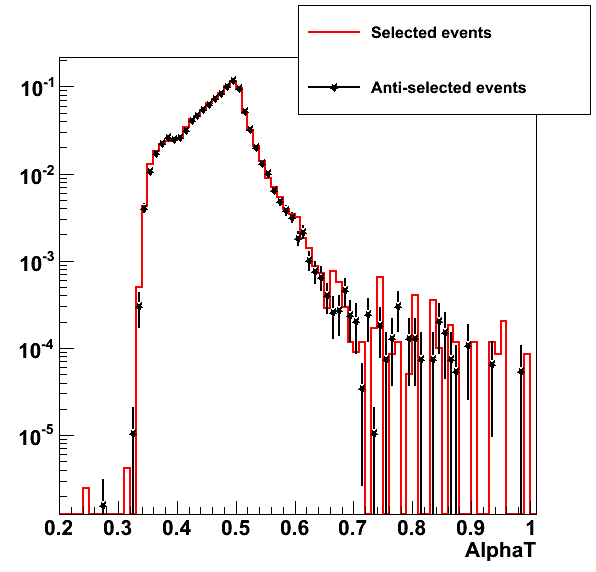
\includegraphics[width=45mm]{leptonicalphaT/alphat_1}
\hspace*{-2mm}
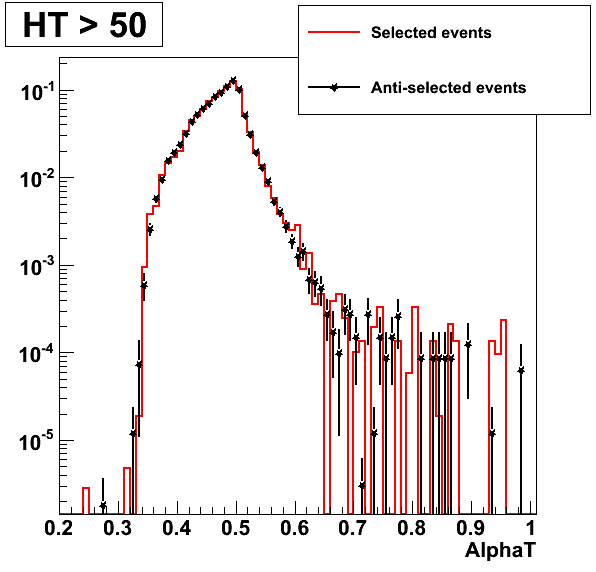
\includegraphics[width=45mm]{leptonicalphaT/alphat_2}
\hspace*{-2mm}
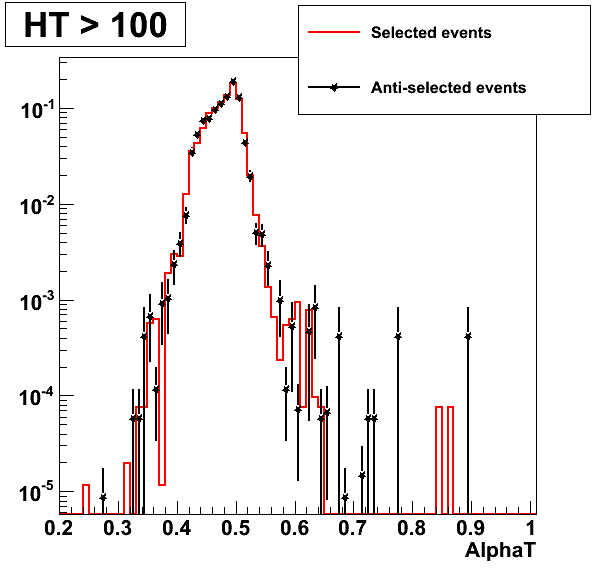
\includegraphics[width=45mm]{leptonicalphaT/alphat_3}
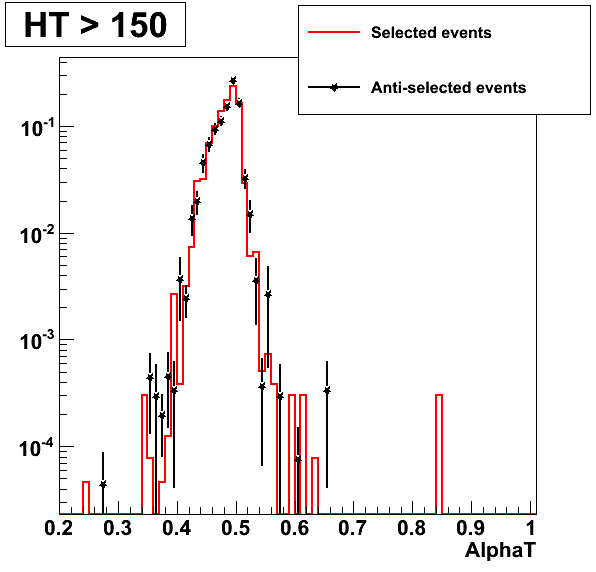
\includegraphics[width=45mm]{leptonicalphaT/alphat_4}
\hspace*{6mm}
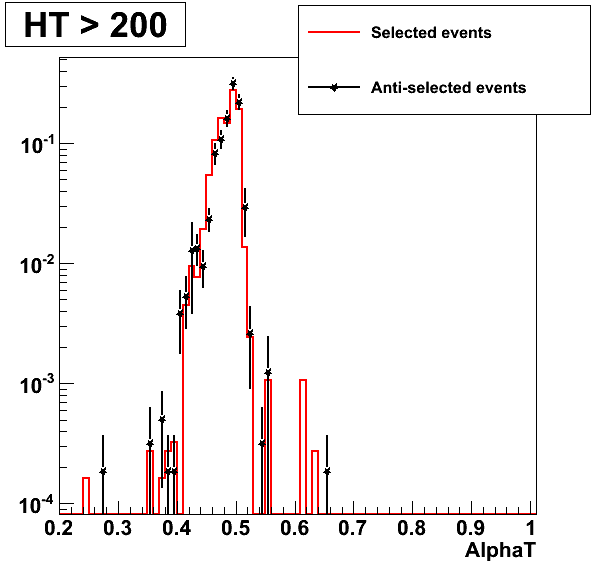
\includegraphics[width=45mm]{leptonicalphaT/alphat_5}
\hspace*{6mm}
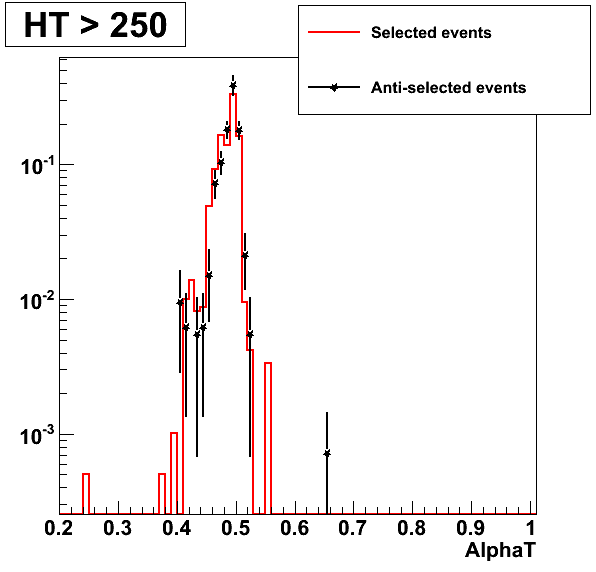
\includegraphics[width=45mm]{leptonicalphaT/alphat_6}
\caption{\textit{The $\alpha_{T}$ distributions for selected (red) and anti-selected events (black) from inversion of the $\Delta \phi$ and $\Delta \eta$ ID Cutts, shown without HT cut (Top Left) and with progressive HT cuts (left-right, top-bottom). These distributions are normalised to unity for shape comparison. There is good agreement between the selected and anti-selected samples regardless of HT requirement, and the high $\alpha_{T}$ tails reduce as expected when moving to higher HT cuts.}}
\label{fig:AlphaTbyHT}
\end{figure}

In order to demonstrate the power of HT in $\alpha_{T}$ tail-reduction, we introduce the variable $R_{\alpha_T}$ which is defined as the ratio of the number of events passing the $\alpha_T$ cut over the number of events failing it:
\begin{equation}
R_{\alpha T} = \frac{N(\alpha_{T}>0.55)}{N(\alpha_{T}<0.55)}
\end{equation}
The ``default'' cut value here is the value prompted from the all-hadronic analysis, 0.55. Figure \ref{fig:AlphaT_Ratio} shows a plot of $R_{\alpha_T}$ as a function of the $H_{T}$ cut applied. As the $H_{T}$ requirement increases, $R_{\alpha_T}$ decreases in an exponential manner. The selected and anti-selected events from the electron id inversion method are in good agreement.

\begin{figure}[h!]
\begin{center}
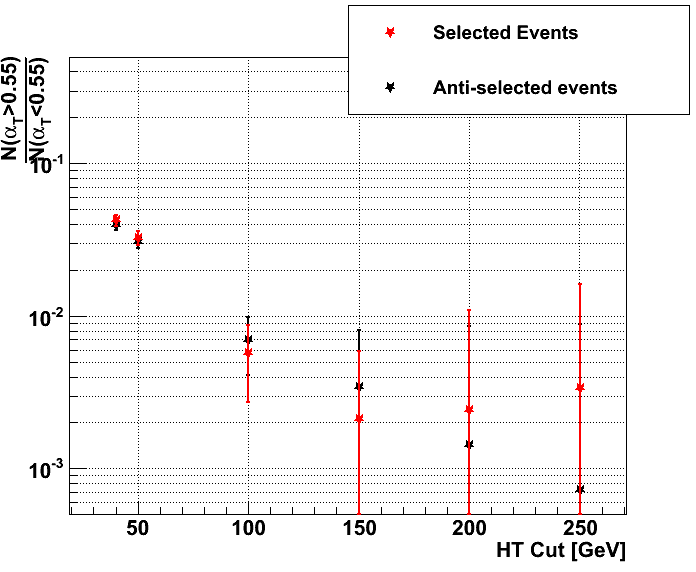
\includegraphics[width=100mm]{leptonicalphaT/AlphaTRatio}
\end{center}
\caption{\textit{The $R_{\alpha_T}$ versus the $H_{T}$ cut applied for the QCD multi-jet background, shown for both selected and anti-selected events in the Delta ID Inversion method.}}
\label{fig:AlphaT_Ratio}
\end{figure}




\end{document}


